%%%%%%%%%%%%%%%%%%%%%%%%%%%%%%%%%%%%%%%%%
% Journal Article
% LaTeX Template
% Version 1.4 (15/5/16)
%
% This template has been downloaded from:
% http://www.LaTeXTemplates.com
%
% Original author:
% Frits Wenneker (http://www.howtotex.com) with extensive modifications by
% Vel (vel@LaTeXTemplates.com)
%
% License:
% CC BY-NC-SA 3.0 (http://creativecommons.org/licenses/by-nc-sa/3.0/)
%
%%%%%%%%%%%%%%%%%%%%%%%%%%%%%%%%%%%%%%%%%

%----------------------------------------------------------------------------------------
%	PACKAGES AND OTHER DOCUMENT CONFIGURATIONS
%----------------------------------------------------------------------------------------

\documentclass[twoside]{article}

\usepackage{blindtext} % Package to generate dummy text throughout this template 
\usepackage{graphicx}

\usepackage[sc]{mathpazo} % Use the Palatino font
\usepackage[T1]{fontenc} % Use 8-bit encoding that has 256 glyphs
\linespread{1.05} % Line spacing - Palatino needs more space between lines
\usepackage{microtype} % Slightly tweak font spacing for aesthetics

\usepackage[english]{babel} % Language hyphenation and typographical rules

\usepackage[hmarginratio=1:1,top=20mm,columnsep=20pt,left=20mm]{geometry} % Document margins
\usepackage[hang, small,labelfont=bf,up,textfont=it,up]{caption} % Custom captions under/above floats in tables or figures
\usepackage{booktabs} % Horizontal rules in tables

\usepackage{lettrine} % The lettrine is the first enlarged letter at the beginning of the text

\usepackage{enumitem} % Customized lists
\setlist[itemize]{noitemsep} % Make itemize lists more compact

\usepackage{abstract} % Allows abstract customization
\renewcommand{\abstractnamefont}{\normalfont\bfseries} % Set the "Abstract" text to bold
\renewcommand{\abstracttextfont}{\normalfont\itshape} % Set the abstract itself to small italic text

\usepackage{titlesec} % Allows customization of titles
\renewcommand\thesection{\Roman{section}} % Roman numerals for the sections
\renewcommand\thesubsection{\roman{subsection}} % roman numerals for subsections
\titleformat{\section}[block]{\large\scshape\centering}{\thesection.}{1em}{} % Change the look of the section titles
\titleformat{\subsection}[block]{\large}{\thesubsection.}{1em}{} % Change the look of the section titles

\usepackage{fancyhdr} % Headers and footers
\pagestyle{fancy} % All pages have headers and footers
\fancyhead{} % Blank out the default header
\fancyfoot{} % Blank out the default footer
\fancyhead[C]{Running title $\bullet$ May 2016 $\bullet$ Vol. XXI, No. 1} % Custom header text
\fancyfoot[RO,LE]{\thepage} % Custom footer text

\usepackage{titling} % Customizing the title section

\usepackage{hyperref} % For hyperlinks in the PDF

%----------------------------------------------------------------------------------------
%	TITLE SECTION
%----------------------------------------------------------------------------------------

\setlength{\droptitle}{-4\baselineskip} % Move the title up

\pretitle{\begin{center}\Huge\bfseries} % Article title formatting
\posttitle{\end{center}} % Article title closing formatting
\title{Party Distributed Processing} % Article title
\author{%
\textsc{Johnson Lam \qquad Justin Chen} \\[1ex] % Your name
\normalsize Boston University \\ % Your institution
% \normalsize \href{mailto:john@smith.com}{john@smith.com} % Your email address
%\and % Uncomment if 2 authors are required, duplicate these 4 lines if more
%\textsc{Jane Smith}\thanks{Corresponding author} \\[1ex] % Second author's name
%\normalsize University of Utah \\ % Second author's institution
%\normalsize \href{mailto:jane@smith.com}{jane@smith.com} % Second author's email address
}
\date{\today} % Leave empty to omit a date
\renewcommand{\maketitlehookd}{%
\begin{abstract}
\noindent In the past few years, machine learning and deep learning have burgeoned from theoretical research to hobbyist computing. Training algorithms require extremely large datasets and users without access to large amounts of resources must purchase them from cloud services, such as AWS, which can be extremely expensive over time. We propose an alternative solution using commodity hardware spread across the internet to tackle this barrier to entry. This could allow any user the opportunity to do computationally intensive work 
\end{abstract}
}

%----------------------------------------------------------------------------------------

\begin{document}

% Print the title
\maketitle

%----------------------------------------------------------------------------------------
%	ARTICLE CONTENTS
%----------------------------------------------------------------------------------------
\section{Introduction}
\lettrine[nindent=0em,lines=3] Open source software libraries, such as TensorFlow, Torch7, and Theano, have made machine learning more accessible than ever before. However, training learning algorithms require massive datasets in the order of several gigabytes to several hundred of gigabytes, which require expensive, specialized GPUs. These models, however, can be just as effectively trained on a large number of CPUs. Cloud services provide these resources at a cost and their interfaces can be
difficult to navigate for new users. 

The average computer is typically under-utilized or idle in a typical day. These available resources could be altruistically allocated to agreed party members for distributed computation. We propose an affordable and easy-to-use distributed data computation paradigm for processing datasets across a party of commodity hardware connected by the internet. Our goal is to lower the cost of entry and simplify the interface users interact with. We use the MapReduce architecture as a guide for our own
design and implement a distributed word counter as a proof-of-concept on BU's csa servers.

%------------------------------------------------
\section{Design}
We propose utililzing hardware owned by a trusted network, like a set of computers owned by a group of friends or a trusted organization. This can even be extended to locally connecting a group of machines that a user accumulates over the years. Our current design utilizes a "master" cloud server that will coordinate work across the party, combine intermediate results from each worker, and return the final result to the client that submitted. Each computer in this network can act a client wanting to do work or as a server available to do work for others. 

Each computer begins by stating their available resources (cores, RAM, etc.) and their restrictions (bandwidth) to the master server when it comes online. At any point in time a computer on the network can make a request to the master server that it'd like to do some work on a dataset and pass the dataset to the master. Similar to how the master node took care of distributing work in MapReduce, the master node in our system will distribute work amongst the available servers in the network based
on each computer's available resources and restrictions. The bottleneck of this design will be the network speed and reliability of each computer. Given this restriction, distribution of work will be in smaller chunks such that sending data over the networkw will not be too cumbersome. The master server will be responsible for handling network failures and unresponsive or slow workers in the same way as if these servers were in the same data center. 

Our current work achieves the abovementioned by distributing work for counting words in a large document, except it does not take into account the available resources and restrictions for a worker. A worker can come and go at any time, and work will be distributed accordingly to this dynamic network inspite of worker failure. The master keeps track of workers currently available to it by sending periodic heartbeats and removes workers from the list who are unresponsive. When
finished, the master returns the final word count to the worker that submitted the request. This implementation is currently running on csa1, csa2, csa3, and ks-sesa with csa1 being the master server. 
%------------------------------------------------
\section{Architecture}
Our program is written in Go and utilizes the "net/http" package to communicate between the worker and master. The master has four endpoints: join, heartbeat, job\_request, and job\_chunk. The worker has three endpoints: heartbeat, process\_chunk, and finish\_job. 

When workers first come online, they notify the master they are joining the network. The worker then idles and waits for either a heartbeat or a job from the master and responds to the master accordingly. When a worker submits a request to the master, the user specifies a URL containing the text document and a name for the document. The worker contributes its resouces for work its given to do by the master. It will then be notified of the final result of its request when the master is finished distributing work. 

The master handles all of the coordination on its fleet of machines. When it first boots up, it starts a thread to send periodic heartbeats to workers that have joined the party. When the master sees a new worker joining, it adds it to its map of current workers and starts a thread responsible for making sure it's responsive by using a timer. If a worker does not respond to a heartbeat, this timer will not be reset and will eventually fire. When the master receives a job
request, it makes a GET request on the URL provided, downloads the page onto its machine, and splits the file up into 1000 line file chunks. It then distributes the file chunks to the available workers, combine their results, and returns it to the submitter

The key components of our work are heartbeating and distribution of work for a request. We use heartbeating as a form of checking on the availability of workers and checking on worker progress on a file chunk. The former case is simple: if the worker is unresponsive after three timeouts, delete the worker. In the latter case, if the worker is unresponsive or fails to make satisfiable progress, delete the worker and add the file chunk back into the queue of jobs that need to be processed. 

We distribute work by creating a separte thread with two channels and treat them as queues, one for jobs to be worked on and one for available and idle workers to process these jobs. We then insert the file chunks and workers into their respective queues. A third channel is used to exit this thread when all jobs have been completed, indicated by when the last file chunk is received. As mentioned earlier, a job is reinserted back into its queue if unsatisfactory progress is made by the worker and the worker is deleted. If a new worker joins in the midst of a request being processed, it adds itself to the worker queue and will
be given a job when one becomes available. When a worker returns the result for a job, the master adds it back into the worker queue. The insertion of jobs and workers into the queue is done on separate thread to ensure that it does not block the master- adding things to the channel will be blocked if a reader is not present on the otherside. The following code illustrates this: 
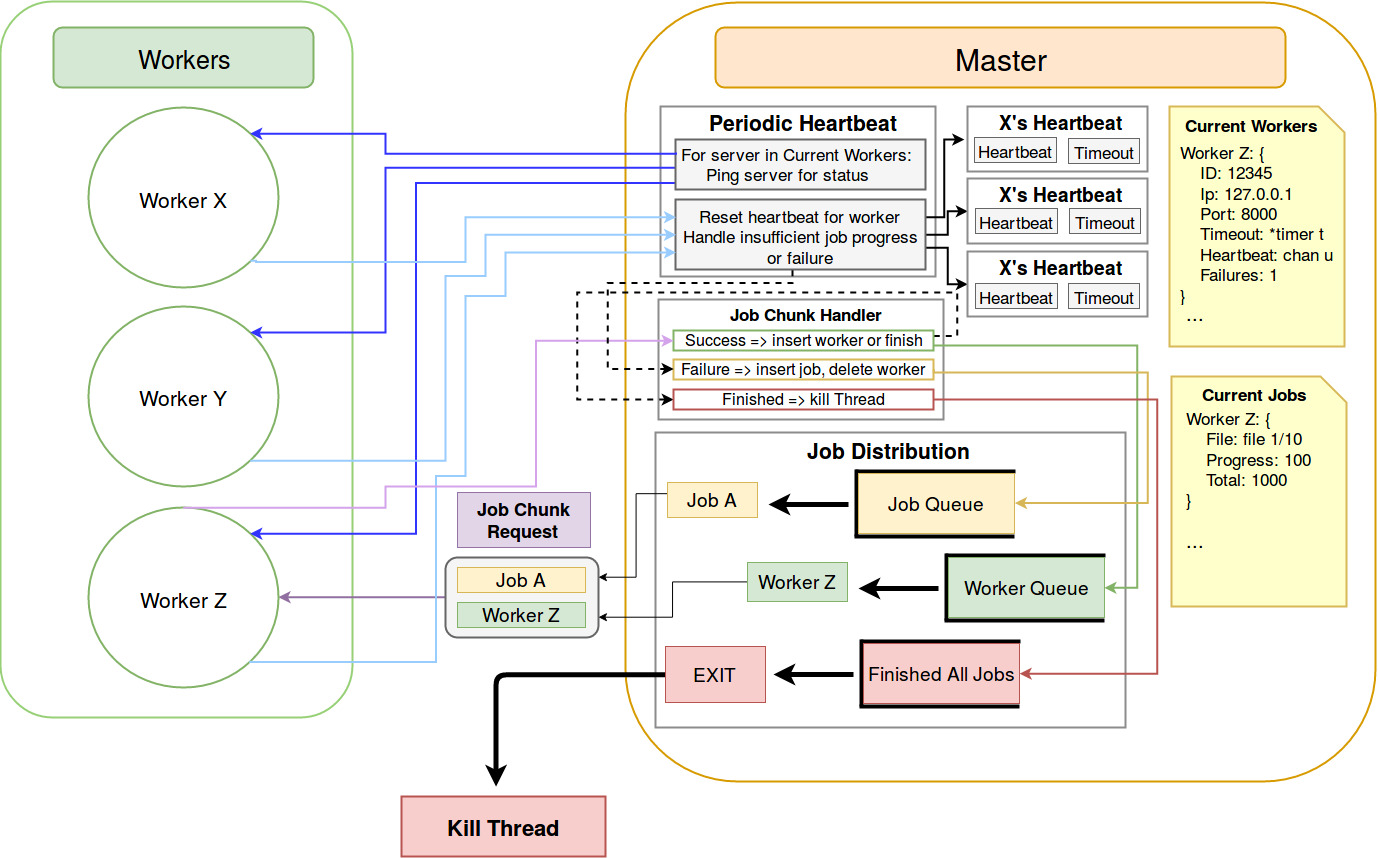
\includegraphics[width=\textwidth]{distribution}
%------------------------------------------------
\section{Benchmarks}
preliminary testing 
further rigorous testing 


%------------------------------------------------

\section{Future Work}

\subsection{Functionality}

\subsection{Architecture}

%----------------------------------------------------------------------------------------
%	REFERENCE LIST
%----------------------------------------------------------------------------------------

\begin{thebibliography}{99} % Bibliography - this is intentionally simple in this template

\bibitem[Figueredo and Wolf, 2009]{Figueredo:2009dg}
Figueredo, A.~J. and Wolf, P. S.~A. (2009).
\newblock Assortative pairing and life history strategy - a cross-cultural
  study.
\newblock {\em Human Nature}, 20:317--330.
 
\end{thebibliography}

%----------------------------------------------------------------------------------------

\end{document}
